\section{Results}\label{sec:results}

\subsection{Sigma Hyperparameter Selection}\label{subsec:sigmaHyperparameterSelectionResults}
Recall that $\sigma_1, \sigma_2, \ldots \sigma_n$ are hyperparameters that must be defined prior to executing the
algorithm.
The grid search exhausts every permutation $P_n^{\sigma_n}$, where:
\begin{equation}
    \label{eq:gridSearchQuerySigma}
    \sigma_n \ \in \ \{10^{-16}, 10^{-15}, \ldots 10^{1}\}
\end{equation}
% 2.22 * 10^-16 is the machine epsilon for double

\begin{figure*}
    \centering{
    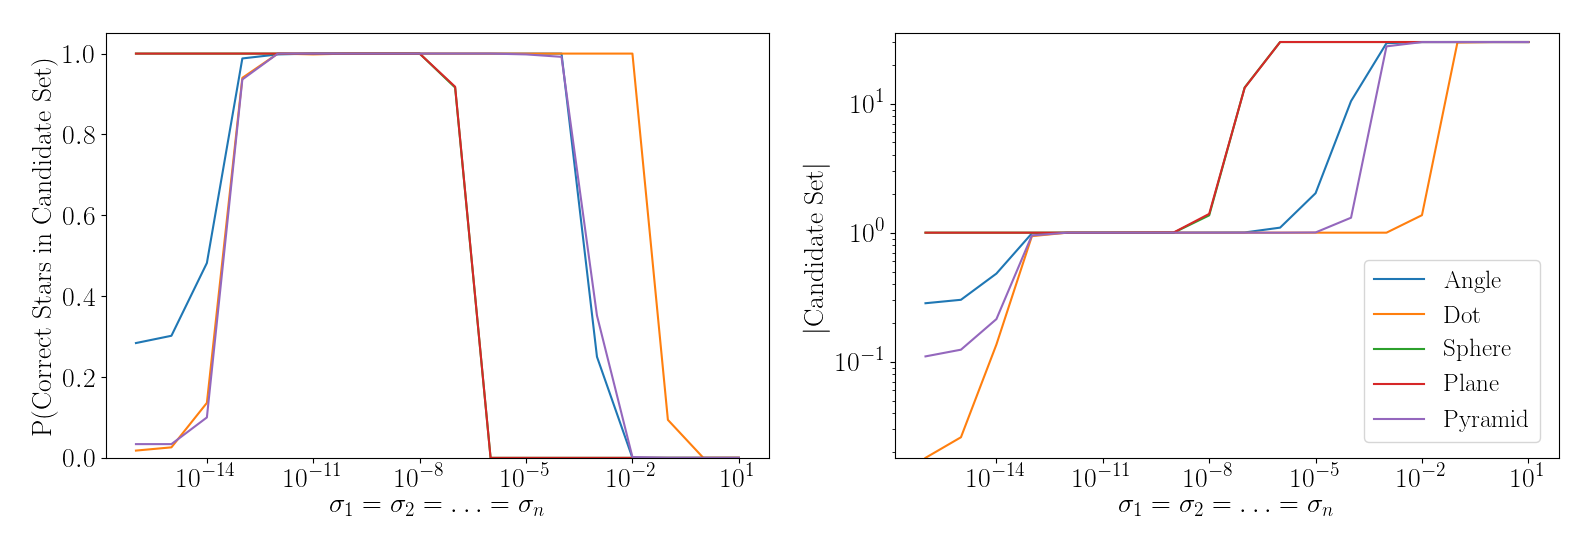
\includegraphics[scale=0.45]{images/sigma1-pcss-css.png}
    \caption{
    The left plot depicts the effect of varying $\sigma$ on the probability that the correct star set exists in the
    resulting candidates after the query.
    The right plot depicts the effect of varying $\sigma$ on the size of the candidate set after the query, bounded
    by 30 candidates at maximum.
    The field-of-view is bounded by $f = 20^\circ$ and the apparent magnitude is bounded by $m = 6.0$.
    Each point represents the average of 500 query steps without noise introduced.
    For brevity, all deviations associated with methods of more than one feature term (i.e.\ Dot Angle, Spherical
    Triangle, \ldots) had all corresponding $\sigma$ terms set equal to each other.
    } \label{figure:sigmaHyperparameterPlots}
    }
\end{figure*}

The set of plots in~\autoref{figure:sigmaHyperparameterPlots} depict the effect on different $\sigma$ terms against the
size of the candidate set $R$ (on the left) and the probability that the correct stars exist in this candidate set (on
the right).
If the deviation is too small, then the selectivity of each query becomes too restrictive and no results are returned.
On the other hand when the selectivity is too high, the candidate set size upper bound of 30 candidates is
hit and the chance that the correct candidate exists in the query declines.

The period of stability for all methods identifying images restricted by $f < 20 \land m < 6.0$ occurs when:
\begin{equation}
    \label{eq:stabilityRegionAcrossFeatures}
    \sigma_n \ \in (10^{-12}, 10^{-8})
\end{equation}
Regardless of the feature, a deviation choice between these bounds should be acceptable for distinguishing stars.

% Not including this, don't feel it is relevant to stability analysis.
%It is important to note that each feature exists in different bounds.
%The values below represent the observed bounds of each feature:
%\begin{alignat*}{2}
%    \label{eq:observedFeatureSpace}
%    % Non-inclusive bounds given below.
%    \theta^{ij} &\in (2.6 \times 10^{-3} &&, 2.0 \times 10^1) \\
%    \theta^{ij} &\in  (2.6 \times 10^{-3} &&, 2.0 \times 10^1) \\
%    \theta^{ic}, \theta^{jc} &\in (2.6 \times 10^{-3} &&, 2.0 \times 10^1) \\
%    \phi &\in (1.3 \times 10^{-3} &&, 1.8 \times 10^2) \\
%    a^{ijk} &\in (3.1 \times 10^{-9} &&, 5.4 \times 10^{-2}) \\
%    \imath^{ijk} &\in (4.8 \times 10^{-16} &&, 5.3 \times 10^{-4}) \\
%    a^{ijk} &\in (3.7 \times 10^{-9} &&, 5.3 \times 10^{-2}) \\
%    \imath^{ijk} &\in (4.9 \times 10^{-16} &&, 5.3 \times 10^{-4})
%\end{alignat*}

\begin{table}
    \centering {
    \caption{
    Query hyperparameter determination stability and sensitivity results of each method.
    The stability length $\ell$ represents the number of deviations where~\autoref{eq:stabilityQuery} is held.
    Each method's critical points $\sigma_{c1}$ and $\sigma_{c2}$ a is the upper bound on the $Q$ and $\lvert R \rvert$
    stability region.
    } \label{tab:sensitivityStabilityResults}
    \begin{tabular}{m{0.27\columnwidth}|m{0.13\columnwidth}|m{0.2\columnwidth}|m{0.2\columnwidth}}
        \textbf{Method} & $\ell$ & $\frac{\partial Q}{\partial\sigma} \text{ at } \sigma_{c1}$ &
        $\frac{\partial \lvert R \rvert}{\partial \sigma} \text{ at } \sigma_{c2}$ \\
        \hline \hline
        \textbf{Angle} & 3 & -0.375 & 0.001 \\ \hline
        \textbf{Dot Angle} & 9 & -0.453 & 0.183 \\ \hline
        \textbf{Spherical \newline Triangle} & 8 & -0.042 & 0.181\\ \hline
        \textbf{Planar \newline Triangle} & 6 & -0.041 & 0.001 \\ \hline
        \textbf{Pyramid} & 7 & -0.001 & 0.002
    \end{tabular}
    }
\end{table}

Referencing~\autoref{tab:sensitivityStabilityResults}, there appears to some correlation between the number of
\textit{distinct} features and length of the stability region here.
The Dot Angle method uses three total features, two of which are distinct from each other ($\theta$ vs. $\phi$) for
it's query.
The Pyramid method uses three similar features, which has the same stable region length as the triangle methods
using two distinct features.
The Angle method uses only one feature for its query, and suffers in stable region length.

The candidate set size responses are most likely a result of the size of possible candidates that belong to each
method's respective feature (i.e.\ the number of rows of the table used in query).
The Angle method has the least number of possible candidates given the $f < 20 \land m < 6.0$ constraint, at 353700
possible catalog sets.
The triangle methods have roughly 35 times as many possible catalog sets as the Angle method.
The Dot Angle method has 3 times as many possible catalog sets as the triangle methods, and roughly 105 times as many
possible catalog sets as the Angle method.
Given a larger pool of results to choose from, it follows that the number of false positive increases as well.

% TODO: How to interpret the Q response?
The largest $Q$ response belongs to the Dot Angle method, while the smallest response belongs to the Pyramid method.
Unlike the candidate set size response, there appears to be no obvious correlation between the response of correct
star set existence and the number of features used.
If noise is not known, the most forgiving feature set in terms of both responses is the Pyramid method.

The $\sigma$ parameters for the following experiments were chosen using the results of the grid search, and selecting
the largest $\sigma_1, \sigma_2, \sigma_3$ (ordered as such) that maintained all the
conditions in~\autoref{eq:stabilityQuery}.
\begin{alignat*}{2}
    \text{Angle}&: \sigma_\theta &&= 1.0 \times 10^{-4}\\
    \text{Pyramid}&: \sigma_\theta &&= 1.0 \times 10^{-4}\\
    \text{Dot Angle}&: \sigma_{\theta_{ic}} &&= 1.0 \times 10^{-1}\\
    \text{Dot Angle}&: \sigma_{\theta_{jc}} &&= 1.0 \times 10^{-1}\\
    \text{Dot Angle}&: \sigma_\phi &&= 1.0 \times 10^{-3} \\
    \text{Spherical Triangle}&: \sigma_a &&= 1.0 \times 10^{-1}\\
    \text{Spherical Triangle}&: \sigma_\imath &&= 1.0 \times 10^{-11}\\
    \text{Planar Triangle / Composite}&: \sigma_a &&= 1.0 \times 10^{-1} \\
    \text{Planar Triangle / Composite}&: \sigma_\imath &&= 1.0 \times 10^{-11}\\
\end{alignat*}

In addition to the $\sigma_n$ parameters used in the previous experiments, a parameter $\sigma_o$ must be defined
prior to executing the \Call{DMT}{} method.
The linear search exhausts every overlay deviation selection:
\begin{equation}
    \label{eq:linearSearchSigmaOverlay}
    \sigma_n \ \in (10^{-16}, 10^{2})
\end{equation}

\begin{figure*}
    \centering{
    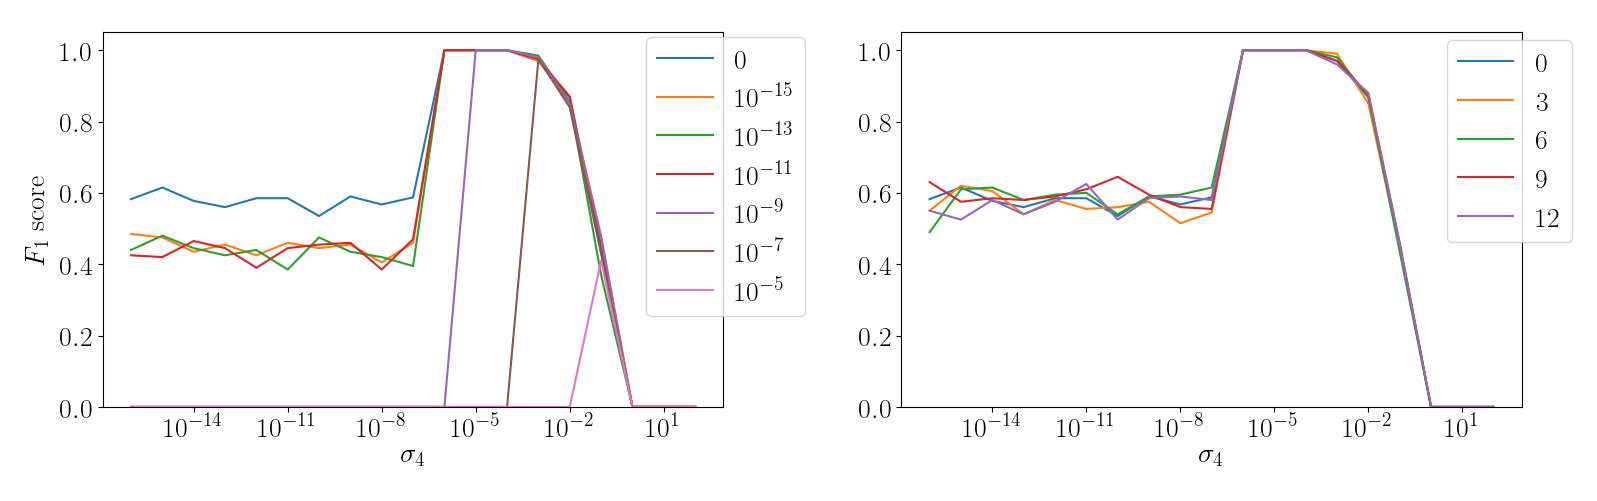
\includegraphics[scale=0.45]{images/sigma4-f1.png}
    \caption{
    Both plots depict the effect of varying $\sigma$ on the F-score.
    The left plot depicts this relationship for different variations in noise, while the right plot depicts the same
    relationship for different numbers of false stars.
    The field-of-view is bounded by $f = 20^\circ$ and the apparent magnitude is bounded by $m = 6.0$.
    Each point represents the average of 200 query steps.
    } \label{figure:sigmaOverlayHyperparameterPlots}
    }
\end{figure*}

The set of plots in~\autoref{figure:sigmaOverlayHyperparameterPlots} depict the effect on different $\sigma$ terms
against the F score.
The period of accurate stability for Gaussian noise under $\sigma = 10^{-5}$ and for all false star introductions occurs
when:
\begin{equation}
    \label{eq:sigmaOverlayStableRegion}
    \sigma_4 \ \in (10^{-6}, 10^{-3})
\end{equation}

% TODO: How to interpret stable region of F = 0.57?
Looking at the both plots it is interesting to note that under no noise (Gaussian or false stars), a $\sigma_4 \ \in
(10^{-17}, 10^{-6})$ gives an $F$ score $~0.57 \pm 1.8 \times 10^{-2}$.
In this region, it appears that the \ldots
On the other end of the stability period for $\sigma_4 > 10^0$, accuracy drops straight to 0 regardless of the noise
presented.
At this period, stars are labeled with more weight to the order of the stars in the imaage rather than actually falling
within the specified deviation.

Focusing on the left plot of varying Gaussian noise, the accuracy dips to zero once the deviation of Gaussian noise
exceeds the selected deviation.
Past the $10^{-4}$ mark, the largest accuracy a deviation choice can achieve is no longer equal to one.
If noise is known, then the appropriate deviation for the \Call{DMT}{} method can be selected.
The right plot shows that the accuracy is not affected under different amounts of false stars.
Given varying amounts of false stars, virtually none of these stars were identified as an actual star.
The \Call{DMT}{} method is seen as highly specific, yielding no false positives.

The value of $\sigma_4 = 10^{-4}$ was selected for use in the \Call{DMT}{} method.
This is the largest deviation that lies in the accurate stable region.

\subsection{Query Selectivity}\label{subsec:querySelectivityResults}
Using the optimal hyperparameters described in the previous section, each query step was analyzed in terms of its
response to an introduction of Gaussian noise.

%\begin{figure*}
%    \centering{
%    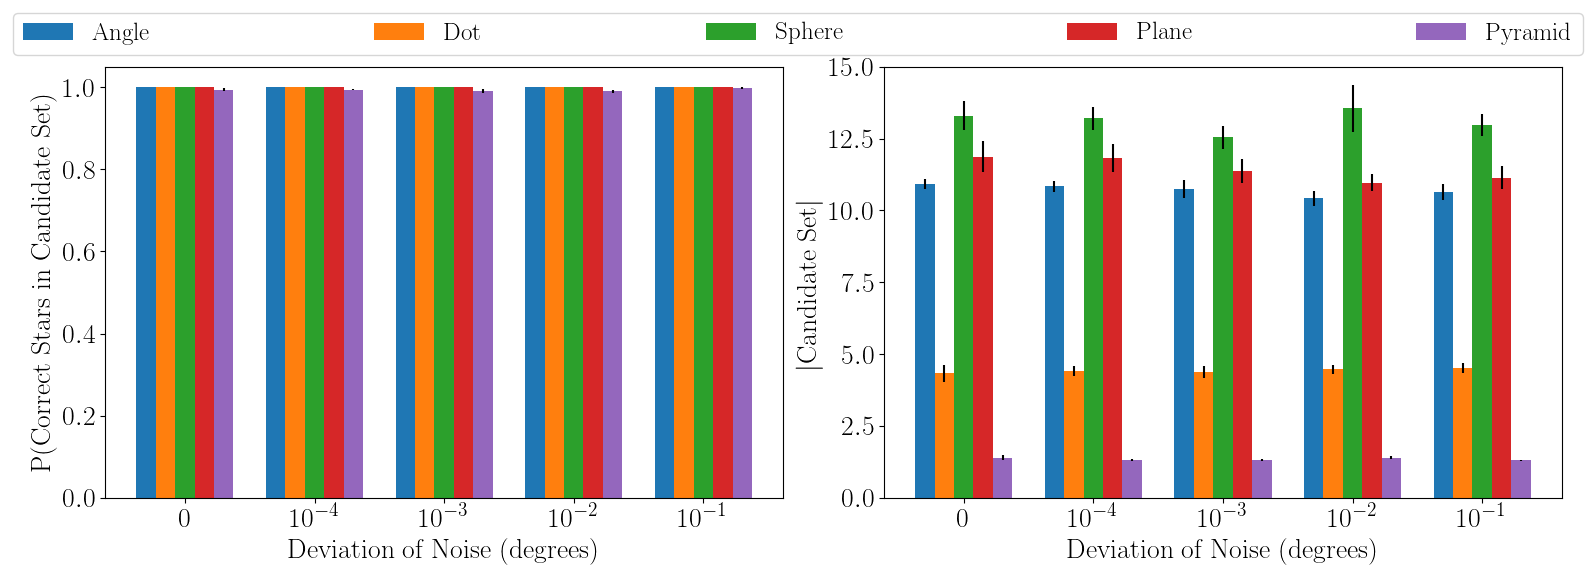
\includegraphics[scale=0.45]{images/query-exp.png}
%    \caption{
%    The left plot depicts the effect of varying the deviation of Gaussian noise on the probability that the correct
%    star set exists in the resulting candidates after the query.
%    The right plot depicts the effect of varying this same noise on the size of the candidate set after the query,
%    bounded by 5000 candidates at maximum.
%    Field of view limit is $f = 20^\circ$.
%    Each point represents the average of 5000 query steps.
%    For the probability measure these 5000 steps were split into 1000 averages, and the mean of these averages are
%    presented above.
%    } \label{figure:queryPlots}
%    }
%\end{figure*}

\begin{table}
    \centering {
    \caption{
    Each method's probability that the correct star set exists after querying ($Q$) and candidate set size under the
    precense of Gaussian noise.
    Every star in the image presented to each identification method's querying process was shifted toward some
    random direction, whose magnitude was normally distributed by $\sigma=0.1^\circ, \mu = 0^\circ$.
    Each point represents the average of five 1000 query steps.
    } \label{tab:queryExperimentResults}
    \begin{tabular}{m{0.18\columnwidth}|m{0.34\columnwidth}|m{0.34\columnwidth}}
        \textbf{Method} & $Q$ & $\lvert R \rvert$ \\
        \hline \hline
        \textbf{Angle} & $1.000 \pm 0.00 $ & $10.90 \pm 1.96 \times 10^{-1}$ \\ \hline
        \textbf{Dot Angle} & $1.000 \pm 0.00 $ & $04.52 \pm 1.08 \times 10^{-1}$ \\ \hline
        \textbf{Spherical \newline Triangle} & $1.000 \pm 0.00 $ & $12.84 \pm 6.61 \times 10^{-1}$ \\ \hline
        \textbf{Planar \newline Triangle} & $1.000 \pm 0.00 $ & $11.43 \pm 2.46 \times 10^{-1}$ \\ \hline
        \textbf{Pyramid} & $0.994 \pm 6.63 \times 10^{-3}$ & $01.31 \pm 2.20 \times 10^{-2}$
    \end{tabular}
    }
\end{table}

In~\autoref{tab:queryExperimentResults}, each method's $Q$ and $\lvert R \rvert$ is displayed under the presence of
noise.
All methods are able to produce no false negatives after the query step except for the Pyramid method, whose accuracy
dips very slightly.
On the other hand, the Pyramid method consistently produces the smallest candidate set size.
By sacrificing $Q$, the Pyramid method ensures a smaller candidate set size.
This tradeoff can only be made when there exists other stars to choose from, as star trackers with a small number of
stars to choose from will be left without other combinations to identify stars from.

The next smallest candidate set size can be seen with the Dot Angle method, followed by the Angle method, and the
triangle methods last.
Feature sets involving angular separation are more selective than those using triangular features.


The most selective feature set that does not sacrifice accuracy is the Dot Angle.

\subsection{Candidate Reduction}\label{subsec:candidateReductionResults}


\subsection{Alignment Determination}\label{subsec:alignmentDeterminationResults}


